\documentclass[11pt]{article}
\usepackage[margin=1in]{geometry}
\usepackage{amsmath,amssymb,amsthm}
\usepackage{graphicx}
\usepackage{hyperref}

\newtheorem*{theorem}{Counterexample}
\newtheorem*{lemma}{Lemma}

\DeclareMathOperator{\conv}{conv}

\title{Divergent orthoprojections in a strictly convex Banach space}
\author{Run fa\_banach\_001, lane 1}
\date{2026-06-14}

\begin{document}
\maketitle

\section*{Source question}

The source paper is Catalin Badea and Yuri I. Lyubich,
\emph{Geometric, spectral and asymptotic properties of averaged products of
projections in Banach spaces}, arXiv:1006.2052.  On page 6, after giving a
divergent example in $\ell_{\infty}^{2}$, the authors write:

\begin{center}
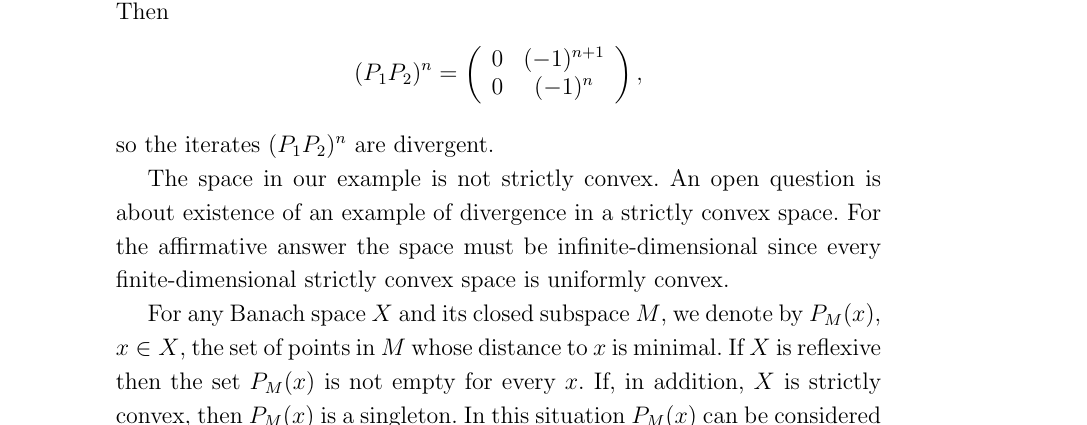
\includegraphics[width=\linewidth]{figures/open_question_crop.png}
\end{center}

In transcription, the question asks whether there is an example of divergence
of iterates of a product of orthoprojections in a strictly convex Banach
space.  Here an orthoprojection means a non-zero norm-one linear projection.

\section*{Proof Intuition}

The two-dimensional $\ell_\infty^2$ example has product eigenvalue $-1$.
Strict convexity forbids such an exact finite-dimensional example, because
finite-dimensional strictly convex spaces are uniformly convex and the source
paper's convergence theorem applies.  But it does not forbid a sequence of
two-dimensional blocks whose product eigenvalues are $-\rho_n^2$ with
$\rho_n\uparrow 1$.

We put these blocks into an $\ell_\infty$-sum.  To make the sum strictly
convex without destroying contractivity of the block projections, we add a
weighted $\ell_2$ term built from the block norms:
\[
  \|x\|=\left(\|x\|_\infty^2+
  \sum_{n=1}^\infty 2^{-n}\|x_n\|_n^2\right)^{1/2}.
\]
The block projections remain contractions for both terms.  The vector
consisting of the distinguished block eigenvectors then witnesses divergence:
for every $m$, some far-out block still has $\rho_n^{4m}$ almost equal to
$1$, so the even and odd powers of the product remain separated.

\begin{lemma}[two-dimensional blocks]
For every $0<\rho<1$ there is a real two-dimensional strictly convex norm
$\|\cdot\|_\rho$ on $\mathbb R^2$ and two norm-one projections $P_\rho,Q_\rho$
such that $P_\rho Q_\rho$ has eigenvalue $-\rho^2$.
\end{lemma}

\begin{proof}
Let
\[
  u_\rho=(1,-\rho),\qquad v_\rho=(\rho,1)
\]
in the coordinate plane with coordinate functionals $e_1^*,e_2^*$.  We first
choose a centrally symmetric strictly convex body $K_\rho$ such that
\[
  \conv\{\pm u_\rho,\pm v_\rho\}\subset K_\rho\subset [-1,1]^2
\]
and $u_\rho,v_\rho\in\partial K_\rho$.

Such a body is obtained by starting with the parallelogram
$\conv\{\pm u_\rho,\pm v_\rho\}$.  Each open side of this parallelogram lies
in the interior of the square $[-1,1]^2$, because $0<\rho<1$.  Replace each
side by a small outward circular arc lying still inside the square, and do so
centrally symmetrically.  The resulting closed convex body has no boundary
line segment, is centrally symmetric, remains inside the square, and keeps
$\pm u_\rho,\pm v_\rho$ on its boundary.  Its Minkowski functional is the
desired strictly convex norm.

Since $K_\rho\subset[-1,1]^2$, the coordinate functionals have norm at most
$1$ for $\|\cdot\|_\rho$.  Since $u_\rho,v_\rho\in\partial K_\rho$, we have
$\|u_\rho\|_\rho=\|v_\rho\|_\rho=1$.  Define
\[
  P_\rho x=e_1^*(x)u_\rho,\qquad Q_\rho x=e_2^*(x)v_\rho.
\]
Then $P_\rho^2=P_\rho$ and $Q_\rho^2=Q_\rho$, and
\[
  \|P_\rho x\|_\rho=|e_1^*(x)|\leq \|x\|_\rho,\qquad
  \|Q_\rho x\|_\rho=|e_2^*(x)|\leq \|x\|_\rho.
\]
Thus $P_\rho$ and $Q_\rho$ are norm-one projections.  Finally,
\[
  Q_\rho u_\rho=-\rho v_\rho,\qquad
  P_\rho Q_\rho u_\rho=-\rho^2 u_\rho,
\]
so $-\rho^2$ is an eigenvalue of $P_\rho Q_\rho$.
\end{proof}

\begin{theorem}
There is a strictly convex real Banach space $X$ and two orthoprojections
$P,Q\in\mathcal B(X)$ such that the iterates $(PQ)^m$ do not converge
strongly.
\end{theorem}

\begin{proof}
Choose $0<\rho_n<1$ with $\rho_n\uparrow 1$.  Let
$E_n=(\mathbb R^2,\|\cdot\|_{\rho_n})$, and let
$P_n=P_{\rho_n}$, $Q_n=Q_{\rho_n}$, and $u_n=u_{\rho_n}$ be as in the lemma.
Let
\[
  Y=\left(\bigoplus_{n=1}^\infty E_n\right)_{\ell_\infty}
\]
with $\|x\|_\infty=\sup_n\|x_n\|_{\rho_n}$.  Define a new norm on $Y$ by
\[
  \|x\|_X=
  \left(
    \|x\|_\infty^2+
    \sum_{n=1}^\infty 2^{-n}\|x_n\|_{\rho_n}^2
  \right)^{1/2}.
\]
This norm is equivalent to $\|\cdot\|_\infty$, hence $X=(Y,\|\cdot\|_X)$ is a
Banach space.

The weighted $\ell_2$ term
\[
  G(x)=\left(\sum_{n=1}^\infty 2^{-n}\|x_n\|_{\rho_n}^2\right)^{1/2}
\]
is strictly convex, because every block norm $\|\cdot\|_{\rho_n}$ is strictly
convex and every block has positive weight.  If equality held in the convexity
inequality for $\|\cdot\|_X$, equality would also hold for $G$, forcing
equality in every non-zero block and hence $x=y$.  Therefore $X$ is strictly
convex.

Define
\[
  P(x_n)=(P_nx_n),\qquad Q(x_n)=(Q_nx_n).
\]
Since each $P_n,Q_n$ is contractive on $E_n$, the operators $P,Q$ are
contractive for both $\|\cdot\|_\infty$ and $G$, hence for $\|\cdot\|_X$.
They are non-zero projections, so $\|P\|=\|Q\|=1$.

Let $T=PQ$ and let $x=(u_n)_{n=1}^\infty\in X$.  Then
\[
  T^m x=\left((-\rho_n^2)^m u_n\right)_{n=1}^\infty.
\]
For each $m\geq 1$,
\[
  T^{2m}x-T^{2m+1}x
  =
  \left(\rho_n^{4m}(1+\rho_n^2)u_n\right)_{n=1}^\infty.
\]
Taking the supremum over $n$ and using $\rho_n\uparrow 1$ gives
\[
  \|T^{2m}x-T^{2m+1}x\|_\infty
  =
  \sup_n \rho_n^{4m}(1+\rho_n^2)=2.
\]
Thus
\[
  \|T^{2m}x-T^{2m+1}x\|_X\geq 2
\]
for every $m$.  The orbit $(T^m x)$ is not Cauchy, so $(PQ)^m$ does not
converge strongly.
\end{proof}

\section*{Complex variant}

The proof above is written over the real field.  If the source question is
read as requiring complex-linear projections, the same construction should be
run with the following balanced version of the two-dimensional block lemma:
inside the closed bidisc of $\mathbb C^2$, take a balanced strictly convex
body whose boundary contains the two circles
\[
  \{\lambda(1,-\rho):|\lambda|=1\},\qquad
  \{\lambda(\rho,1):|\lambda|=1\},
\]
and which is contained in the bidisc.  The same rank-one formulas
$P_\rho z=z_1(1,-\rho)$ and $Q_\rho z=z_2(\rho,1)$ are then complex-linear
contractive projections and the rest of the proof is unchanged.  The real
construction already answers the source paragraph as written; the balanced
variant is included to flag the only extra point for a complex-field review.

\section*{Verification notes}

The only geometric input is the elementary convex-body rounding in the
two-dimensional block lemma.  The rest of the construction is explicit.  The
space is not reflexive and not uniformly convex, as it contains an
$\ell_\infty$-sum structure; this is consistent with the convergence theorem
in the source paper.

A bounded novelty check was performed on 2026-06-14.  The run indexes and
prior archive notes were searched for arXiv:1006.2052, orthoprojections,
strictly convex divergence, and averaged products of projections.  Exact web
searches for the source question and these keywords did not reveal a known
answer.  Novelty confidence is moderate pending human review.

\section*{Human-review recommendation}

Check the planar convex-body block lemma carefully.  If the intended scope is
complex Banach spaces only, check the balanced complex variant stated above.
Once that block lemma is accepted, the infinite-dimensional strictly convex
sum and the divergence calculation are straightforward.

\begin{thebibliography}{9}
\bibitem{BadeaLyubich2010}
Catalin Badea and Yuri I. Lyubich,
\emph{Geometric, spectral and asymptotic properties of averaged products of
projections in Banach spaces},
arXiv:1006.2052, 2010.
\end{thebibliography}

\end{document}
